\documentclass{standalone}
\usepackage{tikz}
\usetikzlibrary{automata, positioning}

\begin{document}
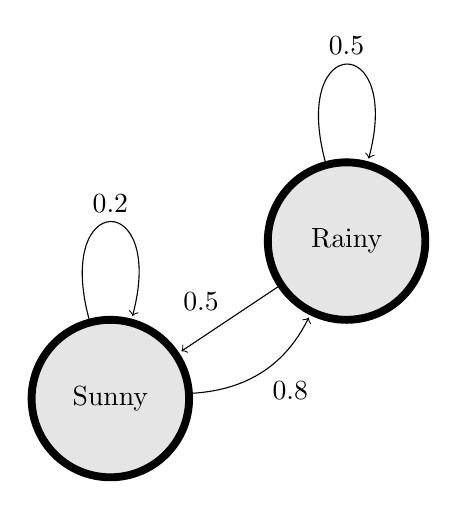
\begin{tikzpicture}


        % Setup the style for the states
        \tikzset{node style/.style={state,
                                    minimum width=2cm,
                                    line width=1mm,
                                    fill=gray!20!white}}


% Add the states
\node[node style] at (0,0) (s) {Sunny};

\node[node style] at (3,2) (r) {Rainy};

	 \draw[every loop]
	  (s) edge[loop above] node {0.2} (s)
		(s) edge[bend right, auto=right] node {0.8} (r)
		(r) edge[auto=right] node {0.5} (s)
		(r) edge[loop above] node {0.5} (r);
\end{tikzpicture}
\end{document}
